\section{Theory}
	\subsection{About the experiment}

		The experimental setup involves a rod pivoted at one end with an LED and a photo-transistor mounted on opposite sides below the pivot point, near the end of the rod (Illustrated in \hyperref[th:1]{Fig 1}). When the rod oscillates through the middle, it blocks the light from the LED to the photo-transistor, generating a pulse. The photo-transistor, being an NPN transistor, gives a spike of current in response to the change in light intensity.

		\begin{figure}
			\centering
			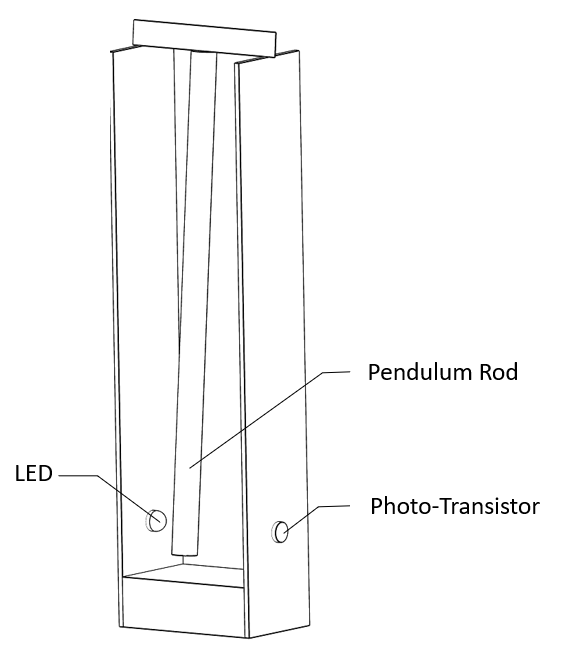
\includegraphics[width=0.6\columnwidth]{images/setup1.png}
			\caption{The experimental setup}
			\label{th:1}
		\end{figure}

		The circuit used in the experiment involves connecting the ground of the LED and the emitter of the photo-transistor to the ground of the Seelab device. The other end of the LED is connected to the PV1 input of the Seelab, while the other end of the photo-transistor is connected to the SEN1 input. Another wire is connected from the SEN1 input to the A1 input of the Seelab. The circuit is shown in \hyperref[th:2]{Fig 2}.

		\begin{figure}
			\centering
			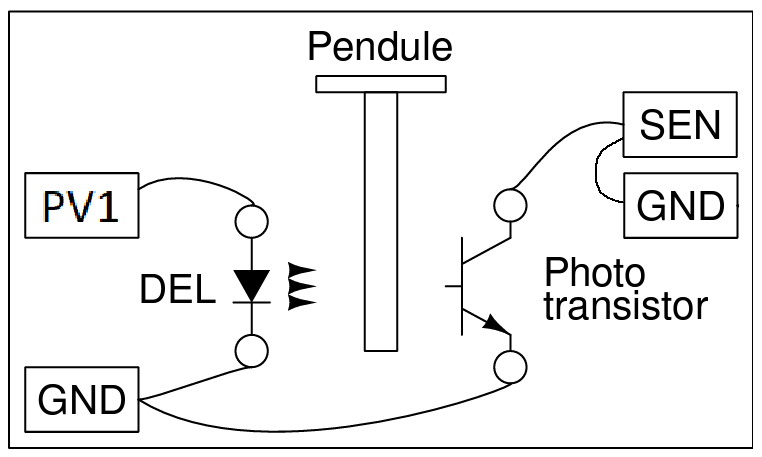
\includegraphics[width=0.8\columnwidth]{images/circuit.png}
			\caption{The Circuit Used}
			\label{th:2}
		\end{figure}

		By capturing the pulses generated by the photo-transistor using the Seelab device, the time period of the oscillations of the pendulum can be measured accurately. This data can then be used to calculate the values of $g$ and $G$, as explained in the theory section. The circuit setup is simple and allows for precise measurements to be made, ensuring accurate results from the experiment.

	\subsection{Calculating the value of gravitational acceleration (g)}

		The time period of an oscillating rod of length $l$ is given by:
		
		$$T = 2\pi \sqrt{\frac{l}{g}}$$
		
		
		For a complex pendulum, the effective length of the pendulum is given by $l_{eff} = \frac{2}{3}l$, where $l$ is the length of the pendulum from the point of suspension to the center of mass. Substituting this value in the above equation, we get:
		
		$$T = 2\pi \sqrt{\frac{2l}{3g}}$$
		
		
		Solving for $g$, we get:
		

		\begin{equation}
			g = \frac{8\pi^2l}{3T^2}
			\label{eq:1}
		\end{equation}


	
	\subsection{The Data}

		We had an NPN photo-transistor. It is an analog output device (output ranging in 0 to 5V) and is characterizes by giving an \texttt{HIGH}er value in shadow and \texttt{LOW}er value in light.

		\begin{figure}[H]
			\centering
			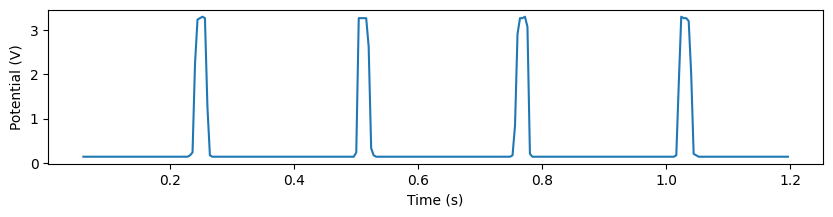
\includegraphics[width=0.8\columnwidth]{images/example_graph.png}
			\caption{How the graph looked (zoomed in time)}
			\label{th:3}
		\end{figure}

		In \hyperref[th:3]{Figure 3}, we can see how a the data plotten on a graph looks like. In x-axis we plot the progression of time, and in y-axis we plot the value output given by the photo-transistor. In the graph we can see a some spikes. Those are created when the pendulum passes through the mean position and casts a shadow on the photo-transistor.